%% LyX 2.1.5 created this file.  For more info, see http://www.lyx.org/.
%% Do not edit unless you really know what you are doing.
\documentclass{article}
\usepackage[T1]{fontenc}
\usepackage{color}
\usepackage{tcolorbox}
\usepackage{amsmath,amssymb,amsthm}
\usepackage{arydshln,mathtools}
\usepackage{diffcoeff}
\usepackage{bm}
\usepackage{url}
\usepackage[footnote]{acronym}
\usepackage[unicode=true,pdfusetitle,
 bookmarks=true,bookmarksnumbered=false,bookmarksopen=false,
 breaklinks=false,pdfborder={0 0 0},backref=false,colorlinks=true]
 {hyperref}
\hypersetup{allcolors=red}

\def\onedot{$\mathsurround0pt\ldotp$}
\def\cdd0ot{% two dots stacked vertically
	\mathbin{\vcenter{\baselineskip.67ex
			\hbox{\onedot}\hbox{\onedot}}%
}}

\DeclareMathOperator{\Tr}{Tr}
\DeclareMathOperator*{\grad}{grad}
\DeclareMathOperator*{\Grad}{Grad}
\DeclareMathOperator*{\Div}{Div}
\renewcommand{\div}{\operatorname{div}}
\DeclareMathOperator*{\Hess}{Hess}

\newcommand{\crmat}[1]{\ensuremath{\widetilde{\left[#1\right]}}}

\makeatletter \renewcommand\d[1]{\ensuremath{%
		\;\mathrm{d}#1\@ifnextchar\d{\!}{}}}
\makeatother

\makeatletter
%%%%%%%%%%%%%%%%%%%%%%%%%%%%%% User specified LaTeX commands.
%===================================
%% --  Page margins
\usepackage{geometry}
\geometry{verbose,twoside,a4paper,
    % Main margins 
top=3cm,
bottom=3cm,
inner=2.5cm,outer=2.5cm,
    % Split of top margins
headheight=2.2cm,headsep=0.5cm,
    % Split of bottom margin
footskip=0.5cm,
    % Split of outer margin
marginparsep=0.5cm,
marginparwidth=12.5pt % width of icon \faNewspaperO at 11pt
}
% Width of icon is computed with
% \newlength{\myl} \settowidth{\myl}{\faNewspaperO} Width of icon \faNewspaperO is \the\myl.
%===================================

%===================================
%% -- Header
%\renewcommand{\thepage}{\roman{page}}% Roman numerals for page counter
\usepackage{fancyhdr}
\pagestyle{fancy}
% Custom fancy style (can be modified on the fly within the document as well)
\fancyhf{} %Clear Everything.
  % Current page number on the exterior
\fancyhead[R]{Brugnoli {\it et al.},  APM-D-18-02037, \thepage}
  % Chapter name on the interior of even pages
\fancyhead[L]{\nouppercase{\leftmark}}
% Redefinition of the plain style
% (This page style is used for the first page of Chapter, table of contents,
% etc...)
\fancypagestyle{plain}{
       \fancyhf{} %Clear Everything.
       \renewcommand{\headrule}{\hrule height 2pt \vspace{1mm}\hrule height 1pt}
       \fancyhead[R]{\thepage}
}
%===================================

%===================================
%% -- tcolorbox to quote
%\usepackage[most]{tcolorbox}
\tcbuselibrary{most}
\tcbuselibrary{breakable} % breakable boxes
%\definecolor{background}{HTML}{F9F5E9}
%\definecolor{linecolor}{HTML}{E0D7BC}
\colorlet{background}{lightgray!80!white}
\colorlet{linecolor}{black}

\newtcolorbox{quotebox}[2][]{%
leftupper=2em,
colback=background,
colframe=background,
%fonttitle=\bfseries,
coltitle=black,
breakable,
enhanced,
attach boxed title to top right,
boxed title style={empty},
sharp corners,
borderline north={0.5pt}{0pt}{linecolor},
borderline north={0.5pt}{1.5pt}{linecolor},
borderline south={0.5pt}{0pt}{linecolor},
borderline south={0.5pt}{1.5pt}{linecolor},
title=#2,#1}

\tcbset{colback=white,
%colframe=green!50!black,
%fonttitle=\bfseries,
coltitle=white,
breakable,enhanced jigsaw,%breakable box
%sharp corners,
}
%===================================

%===================================
%-- 'Remark' and TODO' command
\usepackage{fontawesome}
\usepackage{tcolorbox}
   % enable macro
\newcommand{\remark}[1]{%
\begin{tcolorbox}[title=,colframe=white,colback=lightgray!50!white,fontupper=\sffamily\small]
\faComment~#1
\end{tcolorbox}}
   % disable macro
\renewcommand{\remark}[1]{}
   % enable macro
\newcounter{todocounter}
\newcommand{\todo}[1]{\stepcounter{todocounter}\textbf{\textcolor{red}{(TODO \arabic{todocounter} -- #1)}}}
   % disable macro
%\renewcommand{\todo}[1]{\stepcounter{todocounter} \textbf{ \textcolor{red}{(\arabic{todocounter})} }}
%===================================

%===================================
%%-- Misc.
\usepackage{lipsum}
% Write 'et al.'
% Use \etal (no trailing space) or \etal{} (trailing space)
\newcommand{\etal}{\emph{et al.}}
  % Line numbering
\usepackage{lineno}
\modulolinenumbers[5]
  % For option 'stretch fill image'
\tcbuselibrary{skins}
%===================================

%===================================
%% -- Color for review
   % background color
\colorlet{colorRevBG1}{red!60!black} % dark red
\colorlet{colorRevBG2}{blue!60!black} % dark blue
\colorlet{colorRevBG3}{green!40!black} % dark green
  % front color
\colorlet{colorRev1}{red!80!black} % dark red
\colorlet{colorRev2}{blue!80!black} % dark blue
\colorlet{colorRev3}{green!50!black} % dark green
% Macro to enter revisions
% Usage: \revision[No.]{text}
%\usepackage{ifthen}
\usepackage{xstring}
\newcommand{\revision}[2]{%
\IfStrEqCase{#1}{{1}{\textcolor{colorRev1}{#2}}
    {2}{\textcolor{colorRev2}{#2}}
    {3}{\textcolor{colorRev3}{#2}}}
    [\PackageError{rev}{Unknown reviewer: #1}{Choose available.}]%
}

%===================================

\makeatother

\makeatother

\begin{document}
\thispagestyle{plain}

\noindent {\Large{} MUBO-D-20-00030
}{\Large \par}

\noindent \begin{flushleft}
{\Large{}Port-Hamiltonian flexible multibody dynamics}
\par\end{flushleft}{\Large \par}

\noindent \begin{flushleft}
Andrea Brugnoli, Daniel Alazard, Val\'erie Pommier-Budinger, Denis Matignon
\par\end{flushleft}

\noindent \begin{flushleft}
\today
\par\end{flushleft}

\begin{center}
\textbf{\Large{}Response to reviewers}
\par\end{center}{\Large \par}

We gratefully acknowledge each reviewer for his/her most constructive comments. The quality of the paper has benefited from yours suggestions. Our responses are provided in this document.

Revised passages have been highlighted in the PDF version of the manuscript, with a different color for \textcolor{colorRev1}{Reviewer \#1} and \textcolor{colorRev2}{Reviewer \#2}.

\tableofcontents{}

\section*{Acronyms}

\begin{acronym}[IDA-PBC--] % Specify the longest acronym in order to set the first column width
	\acro{FMS}{\emph{Flexible multibody system}}
	\acro{pH}{\emph{port-Hamiltonian}}
\end{acronym}

\clearpage{}


\section{Summary of revisions}

The manuscript has been revised to account for the comments of the two reviewers. The revisions are highlighted in \revision{1}{red for reviewer \#1} and in \revision{2}{blue for reviewer \#2}. A summary of the revisions
is given below.

\begin{tcolorbox}[title=Summary of revisions (Reviewer No. 1), colframe=colorRevBG1]
\begin{itemize}
\item The introduction has been revised to address comment a, b d.
\item The notation for the cross map has been corrected (comment c).
\item Section 4 has been revised to better illustrate the connection with standard discretization of elasticity problems (comment e).
\item A numerical convergence study has been added to Sec. 6 (comment g and comment 6 of Reviewer 2)
\item The conclusion has been revised in connection to comment h.
\end{itemize}
\end{tcolorbox}


\begin{tcolorbox}[title=Summary of revisions (Reviewer No. 2),colframe=colorRevBG2]
\begin{itemize}
	\item Reference \cite{van2000l2} to answer comment 1. 
	\item Corrections have been made for comments 2, 3, 5.
	\item To addressee comment 4, a remark has been added in Sec. 4.
	\item A convergence study has been added to  section 6. The average cpu time and time step have been added for the examples. 
\end{itemize}
\end{tcolorbox}
 
We have also made the following minor modification: we have introduced the notation 
$$\bm{x}_f := \bm{x} + \bm{u}_f,$$
to compact the equations.

\clearpage{}


\section[Document format]{Format of the present document}


\subsubsection*{Format of response}

An answer is formatted as follows. The reviewer is first quoted with
a gray box that also indicates the position of the quote in the original
review. The comment is then answered in the subsequent paragraph(s).
A description of the revisions and their positions in the unrevised paper is then given in a box.
The color of the box for each reviewer matches the text color used in the revised manuscript, given below.
\begin{itemize}
	\item \textcolor{colorRev1}{Reviewer \#1} 
	\item \textcolor{colorRev2}{Reviewer \#2}
\end{itemize}

\begin{quotebox}{Reviewer No.$i\in\left\{1{,}2\right\} $ -- Position of the quote}
"Direct quote of a comment provided by the reviewer No.$i$."
\end{quotebox}

Answer to the comment for reviewer No. 1.

\begin{tcolorbox}[title=Revision page -- (Reviewer No. $1$),colframe=colorRevBG1]
 Descriptions of the corresponding revisions in the manuscript.
\end{tcolorbox}

Answer to the comment for reviewer No. 2.
\begin{tcolorbox}[title=Revision  page -- (Reviewer No. $2$),colframe=colorRevBG2]
	Descriptions of the corresponding revisions in the manuscript.
\end{tcolorbox}


\subsubsection*{Remark on the use of references}

In our responses, we refer to two families of bibliographic entries:
\begin{itemize}
\item The ones that are contained in the revised manuscript, which are referred
to using the numerical style of the \emph{Journal}, e.g. [1].
\item References\emph{ specific to this document} and not necessarily contained
in the manuscript. To avoid confusion, these references are quoted
using an author-year citation style, e.g. \cite{rong2019}.
\end{itemize}
\clearpage{}


\section{Reply to reviewer \#1}
We thank the reviewer for these detailed and insightful comments. We have addressed each one
below. In the revised manuscript, the corresponding revisions are \textcolor{colorRev1}{highlighted in red}.

\begin{quotebox}{Reviewer No.1 -- Comment a}
	The paper starts with (partially) well known relations on the equations of motion of deformable bodies attached to a reference frame. The PDE-approach is commonly treated in the control theory, but mostly breaks down hereafter by introducing a discretization and some missing links in the otherwise concise derivations. Wouldn't the formulation be much clearer for the reader, if the derivations are shortened by starting with less common approaches?
\end{quotebox}

The equations of motion in Hamiltonian  form can be derived from a variational principle either for rigid body dynamics \cite[Proposition 7.1.1]{holm2008geometric} and general non linear elasticity \cite[Chapter 3]{marsden1981lectures}.  The inclusion of flexibility in case of small deformations using a floating frame formulation is treated in  \cite[Eq. 4.10]{simeon2013computational} using the least action principle. However, in this last reference no comments are made on the Hamiltonian structure of the problem. To the best of our knowledge an Hamiltonian formulation of the floating frame description has not been presented in the literature. It is possible that the equations of motions proposed in the paper can be obtained by means of variational principle, but we have not figured that out yet. For this reason we have simply shown that the equations proposed in \cite{simeon2013computational} can be recast, after some computations, in port-Hamiltonian form. This is neither the clearest nor the most elegant procedure to obtain Sys [12] in the unrevised paper. The final result is anyway consistent with more classical derivations and possesses some nice features. 


\begin{tcolorbox}[title=Revision page 2 and page 28 (Reviewer No. 1 -- Comment a),colframe=colorRevBG1]
Remarks on the Hamiltonian formulation of rigid and general non-linear flexible dynamics have been been made in the introduction (citing \cite[Proposition 7.1.1]{holm2008geometric} and  \cite[Chapter 3]{marsden1981lectures}). 
\end{tcolorbox}


\begin{quotebox}{Reviewer No.1 -- Comment b}
Ref. [39] on page 2 is outdated. There have been much publications since regarding model order reduction related to corotational formulations and inertial/absolute frame.
\end{quotebox}
We agree with this remark and provide a more recent survey on model reduction techniques.


\begin{tcolorbox}[title=Revision pages 2 (Reviewer No. 1 -- Comment b),colframe=colorRevBG1]
The recent review paper \cite{rong2019} has been cited for references on modal reduction strategies for the inertial and corotational frame formulation.
\end{tcolorbox}

\begin{quotebox}{Reviewer No.1 -- Comment c}
	The cross map operator is usually written as a tilde in multibody dynamics.
\end{quotebox}

\begin{tcolorbox}[title=Revision pages --- (Reviewer No. 1 -- Comment c),colframe=colorRevBG1]
	We have adjusted the notation throughout the paper.
\end{tcolorbox}

\begin{quotebox}{Reviewer No.1 -- Comment d}
	While the formulation is really interesting and already commonly used for rigid body systems, I would like to see this formulation for general bodies, not for beams. The concept with beams is what many people treat in robotics, probably in a slightly different manner, but resulting in similar equations (cf. Bremer's projection equations). You state in the abstract "Thanks to the features of the pH framework, complex multibody systems are constructed in a modular way" - but this is the same, if you use the approach from robotics. Do you obtain different equations of motion?
\end{quotebox}
Indeed the numerical applications of the paper only involve beams and this is the reason why a significant part of the paper is dedicated to this specific case. However, this formulation gathers all linear elastic models. For example in the case of the Kirchhoff plate \cite{brugnoli2019kir} one obtains the following system

\begin{equation}
\setlength{\dashlinegap}{2pt}
\bm{\mathcal{E}}
\diffp{}{t}
\underbrace{
	\begin{pmatrix}
	^i \bm{r}_P \\ \bm{R}_{\text{v}} \\ \bm{u}_{m} \\ {u}_{b} \\\hdashline  \bm{v}_P \\ \bm\omega_P  \\ \bm{v}_{m} \\ {v}_{b} \\ \bm{N} \\ \bm{M} \\
	\end{pmatrix}
}_{\bm{e}} = 
\underbrace{
	{\left[ \begin{array}{cccc:cccccc}
		0 & 0 & 0 & 0 &  \bm{R} & 0 & 0 & 0 & 0 & 0 \\
		0 & 0 & 0 & 0 & 0 & \crmat{\bm{R}_{\text{v}}} & 0 & 0 & 0  & 0\\
		0 & 0 & 0 & 0 & 0 & 0 & \bm{I}_{2} & 0 & 0  & 0 \\ 
		0 & 0 & 0 & 0 & 0 & 0 & 0 & 1 & 0  & 0 \\ 
		\hdashline
		-\bm{R}^\top & 0 & 0 & 0 & 0 & \crmat{\widehat{\bm{p}}_t} & 0 & 0  & 0  & 0\\
		0 & -\crmat{\bm{R}_{\text{v}}}^\top & 0 & 0 & \crmat{\widehat{\bm{p}}_t} & \crmat{\widehat{\bm{p}}_r} & \bm{\mathcal{I}}_{p_{m}}^\Omega & \bm{\mathcal{I}}_{p_{b}}^\Omega  & 0  & 0\\
		0 & 0 & -\bm{I}_{2} & 0 & 0 & -(\bm{\mathcal{I}}_{p_{m}}^\Omega)^* & 0 & 0  & \Div  & 0\\
		0 & 0 & 0 & -1& 0 & -(\bm{\mathcal{I}}_{p_b}^\Omega)^* & 0 & 0  & 0  & \div\Div\\
		0 & 0 & 0 & 0 & 0 & 0 & \Grad & 0  & 0  & 0\\
		0 & 0 & 0 & 0 & 0 & 0 & 0 & \Hess  & 0  & 0\\
		\end{array} \right]}
}_{\bm{\mathcal{J}}}
\underbrace{\begin{pmatrix}
	\partial_{\bm{r}_P}H \\ \partial_{\bm{R}_\text{v}}H \\ \delta_{\bm{u}_{m}} H \\ \delta_{u_{b}} H \\\hdashline  \bm{v}_P \\ \bm\omega_P  \\ \bm{v}_{m} \\ {v}_{b} \\ \bm{N} \\ \bm{M} \\
	\end{pmatrix}}_{\bm{z}},
\end{equation} 
where the subscripts $m$ and $b$ denote the membrane and bending contribution, $\bm{u}_{m} \in \mathbb{R}^2, \; {u}_{b} \in \mathbb{R}$ are the in-plane and out-of-plane flexible displacements, $\bm{N} \in \mathbb{R}^{2\times 2}_{\text{sym}}, \; \bm{M} \in \mathbb{R}^{2\times 2}_{\text{sym}}$ the membrane and bending stress resultant. The operator $\div\Div \bm{M} = \sum_{i=1}^{2}\sum_{j=1}^{2} \diffp{M}{x_i,x_j}$ is the double divergence of a tensor and $\Hess$ is the Hessian. The Mindlin plate \cite{brugnoli2019min} results in a larger system that incorporates the flexible angular deflections. The discretization of these model is much harder than that of one-dimensional system. We have recently submitted an ArXiv preprint on this topic \cite{brugnoli2020convergence}. As a linear multibody application involving the Kirchoff plate, we have recently presented \cite{brugnoli2019int} the interconnection of a cantilever plate to a welded rigid bar. \\

Other approaches, commonly used in robotics \cite[Chapter 5]{bremer2008elastic}, allows constructing chain of flexible bodies in a systematic way. However, our approach highlights the Hamiltonian structure and the conservation of energy: the interconnections among bodies do preserve these two important features. \\

The equations of motion we obtain are exactly equivalent to those detailed in \cite{simeon2013computational} and valid only for linear elasticity and moderate angular rotations (since the centrifugal stiffening effect is neglected). The crucial point is that those equations possess an equivalent pH representation.

\begin{tcolorbox}[title=Revision page 3 and pages 9-10 (Reviewer No. 1 -- Comment d ),colframe=colorRevBG1]
	An additional remark has been made in the introduction to cite \cite{bremer2008elastic} for the systematic construction of multibody systems. In the remark at page 8, we have added  a clarification for operators obtained in the Kirchhoff plate .
\end{tcolorbox}


\begin{quotebox}{Reviewer No.1 -- Comment e}
	Eq. (29) is similar to the equations which people often use for flexible multibody dynamics. However, it is hard to see how the according matrices can be computed from the previous derivations. Thus, it would be advantageous, if you interpret these terms with respect to (mechanical) flexible multibody dynamics notation and if you can embed it into existing (common) formulations.
\end{quotebox}
The discretization we use relies on mixed finite elements (cf. \cite{arnold1990mixed} for an interesting introduction), but has a clear connection with the standard discretization. Eq. [29] in the unrevised paper was written compactly for sake of conciseness but indeed it is structured as follows
\begin{equation}\label{eq:findim_mixed}
\begin{bmatrix}
\mathbf{M}_1 & \mathbf{0} \\
\mathbf{0} & \mathbf{M_2} \\
\end{bmatrix}
\begin{pmatrix}
\dot{\mathbf{e}}_1 \\
\dot{\mathbf{e}}_2 \\
\end{pmatrix} = \begin{bmatrix}
\mathbf{0} & -\mathbf{D}^\top \\
\mathbf{D} & \mathbf{0} \\
\end{bmatrix}
\begin{pmatrix}
\mathbf{e}_{1} \\
\mathbf{e}_{2} \\
\end{pmatrix} + 
\begin{bmatrix}
\mathbf{M}_{d}\\
\mathbf{0}\\
\end{bmatrix}
\mathbf{u}_d
+ 
\begin{bmatrix}
\mathbf{B}_{1, \partial}\\
\mathbf{0}\\
\end{bmatrix}
\mathbf{u}_\partial.
\end{equation}

A standard finite element discretization of linear elastodynamics provides a system of the form
\begin{equation}\label{eq:findim_stand}
\mathbf{M}_1 \ddot{\mathbf{q}} + \mathbf{K} \mathbf{q} = \mathbf{M}_{d}\mathbf{u}_d + \mathbf{B}_{1, \partial}\mathbf{u}_\partial,
\end{equation}
where the same notation has been used for identically computed matrices. Since the stiffness matrix $\mathbf{K}$ is symmetric and positive definite, it admits the following non unique factorization \cite{horn2012matrix} (see also \cite[Theorem 2]{cohen2005} for the equivalence of standard and mixed finite elements for elastodynamics problems)
\begin{equation*}
\mathbf{K} = \mathbf{D}^\top \mathbf{M}_2^{-1} \mathbf{D}.
\end{equation*}
Now consider the following variables
\begin{equation*}
\mathbf{e}_1 := \dot{\mathbf{q}}, \qquad 
\mathbf{e}_2 := \mathbf{M}_2^{-1} \mathbf{D}{\mathbf{q}}. 
\end{equation*}
With this change of variables Sys. \eqref{eq:findim_stand} can be equivalently rewritten as \eqref{eq:findim_mixed}.

\begin{tcolorbox}[title=Revision page 12-13 (Reviewer No. 1 -- Comment e ),colframe=colorRevBG1]
	The section 4.1 has been revised to include additional details on the construction of the matrices and the partitioned structure of the final system \ref{eq:findim_mixed}. A remark has been added to compare the standard discretization to the proposed mixed discretization.
\end{tcolorbox}

\begin{quotebox}{Reviewer No.1 -- Comment f}
Eq. (33) should be explained in more detail regarding the $EA^{-1}$ and $EI^{-1}$ terms, which might be natural due to the $\bm{\mathcal{D}}^{-1}$ term in the mass operator, but will be confusing for common readers.
\end{quotebox}

\begin{tcolorbox}[title=Revision page 16 (Reviewer No. 1 -- Comment f ),colframe=colorRevBG1]
	Eq [33] has been commented to explain the presence of the terms $EA^{-1}$ and $EI^{-1}$: these arise in connection to the deformation energy
	\begin{equation*}
	H_{\text{def}} = \frac{1}{2}\int_{0}^L \frac{1}{EA} n_x^2 + \frac{1}{EI} m_x^2  \d\Omega.
	\end{equation*}
\end{tcolorbox}

\begin{quotebox}{Reviewer No.1 -- Comment g}
	I am strongly missing comparison to other formulations and other multibody codes: are the analytical / numerical results the same? Is the performance higher?
\end{quotebox}
The considered numerical examples represent a validation of the proposed formulation with respect to simple benchmark problems available in the literature. The numerical solutions are consistent with publications [14, 18]. \\

 Since the numerical discretization is non standard, we have added a convergence study in Sec. 6 (cf. comment 6 for Reviewer 2). The chosen finite elements exhibit a quadratic convergence in the $H^2$ norm for velocity and displacement and $L^2$ quadratic convergence for the bending stress resultant. \\
 
As far as non linear multibody applications are concerned, we do not claim any computational superiority of this methodology, as we have not analyzed the computational performance  yet.

\begin{tcolorbox}[title=Revision page 21-25 (Reviewer No. 1 -- Comment g ),colframe=colorRevBG1]
	For the four bar mechanism the results of [14] have been plot for comparison. A numerical convergence test has been added to section (cf. comment 6 for Reviewer 2).
\end{tcolorbox}

\begin{quotebox}{Reviewer No.1 -- Comment h}
	I am very much missing the "what does not work" and "restrictions" in the conclusions (e.g., does it work for (flexible) sliding joints or multimodal joints?), which should be present in any "new formulation". The proposed approach starts with a very general PDE formulation, but breaks down to beams in the end. Slider-crank and four bar mechanisms are shown, but no really "complex multibody systems". For those who would like to reproduce the formulation, they have a right to know, if it will work out for their application or it will not.
\end{quotebox}
This formulation works with any kind of rigid joints and could be easily extended for any kind of flexible joints. There are however many points that require further investigations for the simulation of complex multibody systems:
\begin{enumerate}  
\item To address complex multibody systems, higher dimensional models (plates, shells and 3D continua) have to be considered. Port-Hamiltonian plate models and 3D continua are readily available, whereas the reformulation of general shell structures in pH form is still an open topic. For 3D continua and thick plate models (Mindlin-Reissner plates) one may employ the method proposed in \cite{cohen2005} to achieve the discretization. The discretization of thin plate models is substantially more difficult.
\item The employment of finite elements leads to large sparse system to be solved. To limit the computational complexity of these models, model reduction techniques can be incorporated. While for linear pHDAE systems consolidated methodologies exist [15], for the general non linear differential-algebraic case, solutions are not yet available. 
\item To avoid the problem of dealing with large-scale systems, spectral methods can be equivalently used to achieve a structure preserving discretization made up of small and dense matrices.
\item The numerical simulation of the resulting systems have been accomplished using ready-to-use libraries but a rigorous numerical analysis is still to be done. In particular a collocation method based on Gauss-Legendre points exactly preserve the energy balance at a discrete level for pH systems [22, Th. 3]. Collocation methods also works for differential-algebraic pH systems [26]. The application of collocation methods to the proposed framework represents an interesting development.
\end{enumerate}

\begin{tcolorbox}[title=Revision page 28 (Reviewer No. 1 -- Comment h ),colframe=colorRevBG1]
	The conclusion section has been modifies to discuss the points requiring further investigations in connection to the spatial and temporal discretization of the proposed formulation.
\end{tcolorbox}


\clearpage{}

\section{Reply to reviewer \#2}
We thank the reviewer for these constructive comments. We have addressed each one
below. In the revised manuscript, the corresponding revisions are \textcolor{colorRev2}{highlighted in blue}.


\begin{quotebox}{Reviewer No.2 -- Comment 1}
Can the authors explain what they understand by a "lossless" system? It is not a standard term in finite elements technology. 
\end{quotebox}
This term is taken from the control community. A lossless system is a
system that is conservative with respect to the supply rate $s(\mathbf{u}, \mathbf{y}) = \mathbf{u}^\top \mathbf{y}$ (cf. \cite[Definition 3.1.4]{van2000l2}). This means that there exist a storage function $S(t)$ such that
\begin{equation}
	S(t_1) - S(t_0) =  \int_{t_0}^{t_1} \mathbf{u}^\top \mathbf{y} \d{t}.
\end{equation}

For pH (infinite- or finite dimensional) systems with no dissipation the energy rate reads:
\begin{equation*}
	\dot{H} = \mathbf{u}^\top \mathbf{y}.
\end{equation*}
Therefore, the Hamiltonian plays the role of storage function. Integrating between $t_0$ and $t_1$ one obtains
\begin{equation*}
H(t_1) - H(t_0) = \int_{t_0}^{t_1} \mathbf{u}^\top \mathbf{y} \d{t},
\end{equation*}
meaning that the system is lossless.
\begin{tcolorbox}[title=Revision pages10 (Reviewer No. 2 -- Comment 1 ),colframe=colorRevBG2]
The reference \cite{van2000l2} has been cited concerning the definition of lossless system.
\end{tcolorbox}

\begin{quotebox}{Reviewer No.2 -- Comment 2}
The text before equation (21) and (22) does not correspond with equations (21) and (22). Please, rephrase.
\end{quotebox}

\begin{tcolorbox}[title=Revision page 11 (Reviewer No. 2 -- Comment 2 ),colframe=colorRevBG2]
We have revised the text at the indicated location.
\end{tcolorbox}

\begin{quotebox}{Reviewer No.2 -- Comment 3}
	Page (4), before equation (4). Should be infinitesimal STRAIN instead of stress.
\end{quotebox}
\begin{tcolorbox}[title=Revision page 14 (Reviewer No. 2 -- Comment 3),colframe=colorRevBG2]
We performed the necessary correction
\end{tcolorbox}

\begin{quotebox}{Reviewer No.2 -- Comment 4}
Constraints are imposed at the velocity level. It is well-known that a drift appears in this case. Are you using any stabilization ?
\end{quotebox}
No stabilization is used. Imposing the constraints at the velocity level allows preserving the overall pH structure. For linear systems it is possible to use the \textit{Gear-Gupta-Leimkuhler} formulation to preserve the pH structure and enforce the constraints directly on the positions \cite{scholz2019}.

\begin{tcolorbox}[title=Revision page 28 (Reviewer No. 2 -- Comment 4),colframe=colorRevBG2]
In Section 5.2 a remark has been added to address the enforcement of the constraints.
\end{tcolorbox}

\begin{quotebox}{Reviewer No.2 -- Comment 5}
Page 20, first paragraph section 6: four bar MECHANISM.
\end{quotebox}

\begin{tcolorbox}[title=Revision page 21 (Reviewer No. 2 -- Comment 5),colframe=colorRevBG2]
	We performed the necessary correction.
\end{tcolorbox}


\begin{quotebox}{Reviewer No.2 -- Comment 6}
In order to assess about the accuracy of solutions and quality of the approach, it would be important to include a convergence study. What are the typical time steps used in the analyses? Are you getting quadratic convergence ? What are typical cpu times comsumptions for the examples you are displaying ?
\end{quotebox}
The discretization is non-standard as it uses mixed finite elements (cf. \cite{arnold1990mixed} for an interesting introduction). For beam elements, Lagrange polynomial of order one and Hermite polynomials of order 3 are used for $v_f^x$ and $v_f^y$ respectively. Discontinuous Galerkin elements of order 0 and 1 are selected for $n_x$ and $m_{x}$ respectively (see Fig. \ref{fig:fe_beam}). Hermite polynomials guarantee quadratic in the $H^2$ norm for the classical discretization  \cite{hughes2012finite}. With the proposed discretization quadratic convergence in $H^2$ norm is obtained for the displacement and the velocity, while quadratic convergence in the $L^2$
  norm is obtained for the bending stress. \\
  
Constructing stable finite elements in higher dimensions is more difficult. For additional information on the topic, our recent ArXiv preprint on the discretization of plate models \cite{brugnoli2020convergence} can be consulted.
 
 \begin{figure}[t]
 	\centering
 	\includegraphics[width=0.8\textwidth]{fe_beam.eps} \hspace{.5cm}
 	\caption{Finite element choice for Euler Bernoulli beams.}
 	\label{fig:fe_beam} The notation $\mathcal{P}_k$ indicates the space of polynomials of degree $k$.
 \end{figure}

\begin{tcolorbox}[title=Revision page 10 (Reviewer No. 2 -- Comment 6),colframe=colorRevBG2]
	In Sec. 6 we have added a convergence study with respect to an analytic solution for the vertical vibration of a simply supported beam. The average cpu time and time step have been added for the crank slider and rotating beam tests.
\end{tcolorbox}


\clearpage{}


\bibliographystyle{alpha}
\bibliography{biblio}
\end{document}
